\documentclass[math0540-lecture-notes.tex]{subfiles}
\begin{document}

\chapter{Inner Product Spaces}

With vector spaces, we generalized the linear structure (of addition and scalar multiplication) in
$\R^2$ and $\R^3$; however, we ignored other important features, such as length and angle. We now
explore these ideas through \textbf{inner products}.

\section{Inner Products and Norms}
\subsection{Inner Products}

To motivate inner products, let's recall vectors in $\R^2$. The length of a vector $\vec{v}\in \R^2$
is called the \textbf{norm} of $\vec{v}$, denoted $\|\vec{v}\|$; and we calculate the norm of a
vector $\vec{v}=(x_1,x_2)$ as follows: \[
  \|\vec{v}\|=\sqrt{x_1^2+x_2^2}
.\] Similarly, if $\vec{v}=(x_1,x_2,x_3)\in \R^3$, then \[
  \|\vec{v}\|=\sqrt{x_1^2+x_2^2+x_3^2}
.\] Even though we can't visualize vectors in higher dimensions, the generalization to $\R^n$ is
clear: for a vector $\vec{v}=(x_1,x_2,\ldots,x_n)\in \R^n$, the norm of $\vec{v}$ is \[
  \|\vec{v}\|=\sqrt{x_1^2+x_2^2+\ldots+x_n^2}
.\] However, clearly the norm is not linear on $\R^n$. To achieve this linearity, we introduce the
\textbf{dot product}.

\begin{definition}[Dot Product]{}
  For $x,y\in \R^n$, the \textbf{dot product} of $x$ and $y$, denoted $x\cdot y$, is \[
    x\cdot y=x_1y_1+\ldots+x_ny_n
  ,\] where $x=(x_1,\ldots,x_n)$ and $y=(y_1,\ldots,y_n)$.
\end{definition}

Importantly, the dot product of two vectors of $\R^n$ is a number, \textbf{not} a vector. Clearly,
\[
  x\cdot x=\|x\|^2
\] for all $x\in \R^n$. The dot product has the following properties:
\begin{itemize}
  \item $x\cdot x\ge 0$ for all $x\in \R^n$.
  \item $x\cdot x=0$ if and only if $x=0$.
  \item For $y\in \R^n$ fixed, the map from $\R^n$ to $\R$ that sends $x\in \R^n$ to $x\cdot y$ is
    linear.
  \item $x\cdot y=y\cdot x$ for all $x,y\in \R^n$.
\end{itemize}

Now, how might we generalize the dot product from $\R^n$ to a general vector space? An intuitive
notion may simply be to abstract the properties listed above. However, while this works for real
vector spaces, we want a definition that works for complex vector spaces as well. We introduce the
notion of \textbf{inner products}, but first, a review of complex numbers.

\begin{definition}[Complex Conjugates]{}
  Suppose $z=a+bi\in \C$. The \textbf{complex conjugate of $z$}, denote $\overline{z}$, is defined
  as \[
    \overline{z}=a-bi\in \C
  .\] Thus $z=\overline{z}$ if and only if $z\in \R$, i.e. $z=a+0i$ for some $a\in \R$.
\end{definition}

Note that complex conjugates respect addition and multiplication, in that \[
  \overline{z+w}=\overline{z}+\overline{w} ~\text{and}~ \overline{zw}=\overline{z}\overline{w}
\] for $z,w\in \C$. In other words, complex conjugation is an isomorphism between complex numbers.

\begin{definition}[Norm of Complex Number]{}
  The \textbf{absolute value}, or \textbf{norm}, of $z=a+bi$ is \[
    \left| z \right| =\sqrt{a^2+b^2}=\sqrt{(a+bi)(a-bi)}=\sqrt{z\overline{z}}
  .\] 
\end{definition}
Absolute values respect multiplication, i.e. $\left| zw \right| =\left| z \right| \left| w \right|$,
but \textbf{not} addition! See the section on triangle inequalities for absolute values and
addition.




\begin{definition}[Inner Product]{}
  An \textbf{inner product} on $V$ is a function that takes each ordered pair $(u,v)$ of elements of
  $V$ to a number $\left<u,v \right>\in \F$ and has the following properties:
  \begin{itemize}
    \item \textbf{Positive Definiteness}: $\left<v,v \right> \ge 0$ for all $v\in V$, and $\left<v,v
      \right>=0$ if and only if $v=0$.
    \item \textbf{Conjugate Symmetry}: $\left<u,v \right> = \overline{\left<v,u \right>}$ for all
      $u,v\in V$ (note that every real number equals its complex conjugate).
    \item \textbf{Linearity}: $\left<u+v,w \right> = \left<u,w \right>+\left<v,w \right>$ for all
      $uv,w\in V$, and $\left<\lambda u,v \right>=\lambda\left<u,v \right>$ for $\lambda\in \F$.
  \end{itemize}
\end{definition}

\begin{example}
  Here are some examples of inner products:
  \begin{itemize}
    \item The \textbf{Euclidean inner product} on $\F^n$, defined by \[
        \left<(w_1,\ldots,w_n),(z_1,\ldots,z_n) \right>=w_1\overline{z_1}+\ldots+w_n\overline{z_n}
      .\] If $\F$ is real, this is simply the dot product. If $c_1,\ldots,c_n$ are positive numbers,
      then the Euclidean inner product can be extended to \[
          \left<(w_1,\ldots,w_n),(z_1,\ldots,z_n)
          \right>=c_1w_1\overline{z_1}+\ldots+c_nw_n\overline{z_n}
      .\] 
  \item An inner product can be defined on the vector space of continuous real-valued functions on
    the interval $[-1,1]$ by \[
      \left<f,g \right>=\int_{-1}^1 f(x)g(x)dx
    .\] With polynomials, a similar inner product may be defined \[
    \left<p,q \right> = \int_0^\infty p(x)q(x)e^{-x}dx
    .\] 
  \end{itemize}
\end{example}

Inner products exist over vector spaces; we give these vector spaces a name.
\begin{definition}[Inner Product Spaces]{}
  An \textbf{inner product space} is a vector space $V$ along with an inner product on $V$.
\end{definition}

The most prominent example of an inner product space is $\F^{n}$ with the Euclidean inner product,
as defined above. When $\F^{n}$ is referred to as an inner product space, assume the inner product
is the Euclidean inner product unless explicitly told otherwise.

For notational convenience, too, we now denote $V$ an inner product space over $\F$.

\begin{proposition}[Properties of Inner Products]{}
  \begin{itemize}
    \item For each fixed $u\in V$, the function that takes $v$ to $\left<v,u \right>$ is a linear
      map from $V$ to $\F$.
    \item $\left<0,u \right>=0$ for every $u\in V$.
    \item $\left<u,0 \right> = 0$ for every $u\in V$.
    \item $\left<u,v+w \right> = \left<u,v \right>+\left<u,w \right>$ for all $u,v,w\in V$. For
      $\lambda\in \F$, $\left<u,\lambda v \right>=\overline{\lambda}\left<u,v \right>$. In other
      words, an inner product is \textbf{conjugate-linear} in the second term.
  \end{itemize}
\end{proposition}
\begin{proof}[Proof]
  (1) follows from the conditions of linearity in the first term for inner products. (2) follows
  from (1), since every linear map takes $0$ to $0$. (3) follows from (1) and the conjugate symmetry
  property of linear maps.

  For (4), suppose $u,v,w\in V$. Then
  \begin{align*}
    \left<u,v+w \right> &= \overline{\left<v+w,u \right>} \\
                        &= \overline{\left<v,u \right>+\left<w,u \right>} \\
                        &= \overline{\left<v,u \right>}+\overline{\left<w,u \right>} \\
                        &=\left<u,v \right>+\left<u,w \right>
                      .\end{align*} For (5), suppose $u,v\in V,\ \lambda\in \F$. Then
  \begin{align*}
    \left<u,\lambda v \right> &= \overline{\left<\lambda v,u \right>} \\ 
    &= \overline{\lambda\left<v,u \right>} \\
    &= \overline{\lambda} \overline{\left<v,u \right>}\\
    &=\overline{\lambda}\left<u,v \right>
  .\end{align*}
\end{proof}

\subsection{Norms}

Our motivation for defining inner products came initially from the norms of vectors in $\R^2$ and
$\R^3$, which represented the ``length'' of a vector. Now, we see that each inner product determines
a norm.
\begin{definition}[Norm]{}
  For $v\in V$, the \textbf{norm} of $v$, denoted $\|v\|$, is defined by \[
    \|v\|=\sqrt{\left<v,v \right>}
  .\] 
\end{definition}

Example norms include the standard norm on $\F^{n}$, where \[
  \|(z_1,\ldots,z_n)\|=\sqrt{\left| z_1 \right|^2+\ldots+\left| z_n \right| ^2 }
.\] In the vector space of continuous real-valued functions on $[-1,1]$ (with inner product defined
above), we have \[
  \|f\|=\int_{-1}^{1}(f(x))^2dx 
.\]

Now, let's look at some basic properties of norms.
\begin{proposition}[Properties of Norms]{}
  Suppose $v\in V$.
  \begin{enumerate}
    \item $\|v\|=0$ if and only if $v=0$.
    \item $\|\lambda v\|=\left| \lambda \right| \|v\|$ for all $\lambda\in \F$.
  \end{enumerate}
\end{proposition}
\begin{proof}[Proof]
  (1) follows directly from inner products, since $\left<v,v \right> = 0$ if and only if $v=0$.
  Suppose $\lambda\in \F$. Then
  \begin{align*}
    \|\lambda v\|^2&=\left<\lambda v,\lambda v \right>\\
                   &= \lambda\left<v,\lambda v \right>\\
                   &=\lambda\overline{\lambda}\left<v,v \right>\\
                   &=\left| \lambda \right| ^2\|v\|^2
  .\end{align*} Taking square roots now gives the desired equality.
\end{proof}

The above proof also illustrates that in general, working with norms squared is usually easier than
working directly with norms.

Now, we come to a crucial definition.
\begin{definition}[Orthoganl]{}
  Two vectors $u,v\in V$ are \textbf{orthogonal} if $\left<u,v \right> =0$.
\end{definition}
Order does not matter here, because $\left<u,v \right>=0$ if and only if $\left<v,u  \right> = 0$
(by properties of conjugates).  We also sometimes say $u$ is orthogonal to $v$. One should check
that if $u,v$ are non-zero vectors in $\R^2$, then \[
  \left<u,v \right> = \|u\|\|v\|\cos{\theta}
,\] where $ \theta$ is the angle between $u$ and $v$. This aligns with our intuition; two vectors in
$\R^2$ are orthogonal if the angle between them is $90^{\circ}$. In other words, \textit{orthogonal}
is a fancier, abstracted notion of \textit{perpendicular}.

Let's look at some basic properties of orthogonality.
\begin{proposition}[Orthogonality and $0$]{}
  \begin{itemize}
    \item $0$ is orthogonal to every vector in $V$.
    \item $0$ is the only vector in $V$ that is orthogonal to itself.
  \end{itemize}
\end{proposition}
\begin{proof}[Proof]
  Recall from earlier that $\left<0,u \right> =0$ for every $u\in V$. Additionally, if $v\in V$,
  and $\left<v,v \right> =0$, by positive definiteness we need $v=0$.
\end{proof}

Orthogonality can also be used to prove a familiar theorem:
\begin{theorem}[Pythagorean Theorem]{}
  Suppose $u,v\in V$ are orthogonal. Then \[
    \|u+v\|^2=\|u\|^2+\|v\|^2
  .\] 
\end{theorem}
\begin{proof}[Proof]
  \begin{align*}
    \|u+v\|^2&= \left<u+v,u+v \right> \\
             &= \left<u,u \right> +\left<u,v \right>+\left<v,u \right>+\left<v,v \right>\\
             &= \left<u,u \right>+\left<v,v \right> \\
             &=\|u\|^2+\|v^2\|
  .\end{align*}
  We get the second last step because orthogonality implies $\left<u,v \right> = \left<v,u \right> =
  0$.
\end{proof}

Now, suppose $u,v\in V$ with $v\neq 0$. We would like to write $u$ as a scalar multiple of $v$, plus
a vector $w$ orthogonal to $v$:
\begin{figure}[htpb]
  \centering
  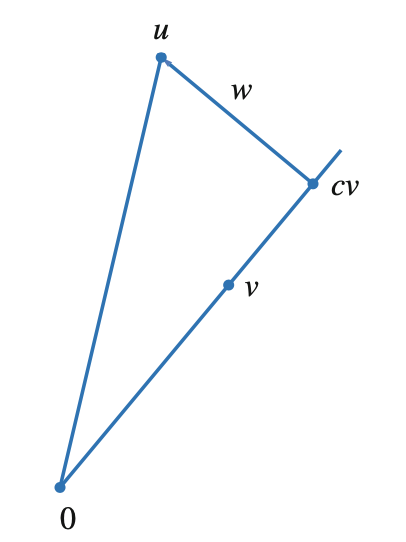
\includegraphics[width=0.25\textwidth]{axler6adecomp.png}
\end{figure}
In other words, we would like to \textit{decompose} $u$ into a vector $v$, plus some vector
orthogonal to $v$.

To do this, let $c\in \F$ denote a scalar. Then \[
  u = cv+(u-cv)
.\] Thus we need to choose $c$ so that $v$ is orthogonal to $u-cv$. In other words, we need \[
  0 =\left<u-cv,v \right> =\left<u,v \right> - c\left<v,v \right> =\left<u,v \right>-c\|v\|^2
.\] From this, we want \[
  c = \frac{\left<u,v \right>}{\|v\|^2}
.\] So, we can decompose $u$ into a scaled vector $v$, plus a vector $w=u-\frac{\left<u,v
\right>}{\|v\|^2}$ orthogonal to $v$: \[
  u = \frac{\left<u,v \right>}{\|v\|^2}v+\left(u-\frac{\left<u,v \right>}{\|v\|^2}v\right)
.\] In other words, we have proved the following result:
\begin{proposition}[Orthogonal Decomposition]{}
  Suppose $u,v\in V$ with $v\neq 0$. Set $c=\frac{\left<u,v \right>}{\left<v,v
  \right>}=\frac{\left<u,v \right>}{\|v\|^2}$, and $w=u-cv$. Then \[
    \left<w,v \right>=0 ~\text{and}~u=cv+w
  .\] 
\end{proposition}

If we only look at $cu$, this is essentially the value of the vector $v$ if \textbf{projected} onto
the vector $u$; that is, if we look at the value of $v$ only on $u$. This process has a special
name:
\begin{definition}[Gram-Schmidt Process]{}
  Let $u,v\in V$ with $v\neq 0$. The \textbf{projection of $v$ onto $u$}, denoted $\proj_{v}(u)$, is
  defined by \[
    \proj_{v}(u)=\frac{\left<u,v \right>}{\left<v,v \right>}v
  .\] [Gram-Schmidt Process, postponed.]
\end{definition}

Orthogonal decomposition is quite useful, especially in the proof of the following important
equality:
\begin{proposition}[Cauchy-Schwarz Inequality]{}
  Suppose $u,v\in V$. Then \[
    \left| \left<u,v \right> \right|  \le \|u\|\|v\|=\left<u,u \right>\left<v,v \right>
  .\] Equality holds if and only if one vector is a scalar multiple of another.
\end{proposition}
\begin{proof}[Proof]
  If $v=0$, then both sides of the desired inequality equal $0$, so suppose $v\neq 0$. Consider \[
    u = \frac{\left<u,v \right>}{\left<v,v \right>}v+w
  \] given above, where $w$ is orthogonal to $v$. By the Pythagorean Theorem,
  \begin{align*}
    \|u\|^2&= \|\frac{\left<u,v \right>}{\left<v,v \right>}v\|^2+\|w\|^2 \\
           &= \frac{\left| \left<u,v \right> \right| ^2}{\left<v,v \right>}+\|w\|^2 \\
           &\ge \frac{\left| \left<u,v \right> \right| ^2}{\|v\|^2}
  .\end{align*} Hence \[
    \|u\|^2\|v\|^2 \ge \left| \left<u,v \right> \right| ^2
  ,\] and taking square roots then gives us the desired inequality.

  From the above proof, Cauchy-Schwarz is an equality if and only if this statement is an equality:
  \[
    \frac{\left| \left<u,v \right> \right| ^2}{\left<v,v \right>}+\left<w,w \right>\ge \frac{\left|
    \left<u,v \right> \right|^2 }{\left<v,v \right>}
  .\] Clearly, this is true only when $\left<w,w \right>=0$, or $w=0$. But $w=0$ if and only if $u$
  is a multiple of $v$ (geometrically, the orthogonal vector between $u$ and $v$ is $0$ only when
  one is a multiple of another). Thus equality holds if and only if one vector is a scalar multiple
  of another.
\end{proof}

The next result, called the \textbf{Triangle Inequality}, has the geometric interpretation that the
length of each side of a triangle is less than the sum of the lengths of the other two sides. This
also implies that the shortest path between two points is a line segment.

\begin{proposition}[Triangle Inequality]{}
  Suppose $u,v\in V$. Then \[
    \|u+v\|\le \|u\|+\|v\|
  .\] Again, equality holds if and only if one of $u,v$ is a non-negative multiple of another.
\end{proposition}
\begin{proof}[Proof]
  We have
  \begin{align*}
    \|u+v\|^2&= \left<u+v,u+v \right> \\
             &= \left<u,u \right>+\left<u,v \right>+\left<v,u \right>+\left<v,v \right> \\
             &= \left<u,u \right>+\left<v,v \right>+\left<u,v \right> +\overline{\left<u,v \right>}\\
             &\le  \|u\|^2+\|v\|^2+2\left| \left<u,v \right> \right|  \\
             &\le \|u\|^2+\|v\|^2+2\|u\|\|v\| \\
             &= (\|u\|+\|v\|)^2
  .\end{align*}
  The second last inequality comes from the Cauchy-Schwarz Inequality, and taking square roots thus
  gives the desired inequality: \[
    \|u+v\|\le \|u\|+\|v\|
  .\] 

  Equality holds if and only if $\left<u,v \right> =\|u\|\|v\|$; but this only holds if one is a
  scalar multiple of another. 
\end{proof}

This final result is called the parallelogram equality, because of its geometric interpretation: in
every parallelogram, the sum of the squares of the lengths of the diagonals equals the sum of the
squares of the lengths of the four sides.
\begin{figure}[htpb]
  \centering
  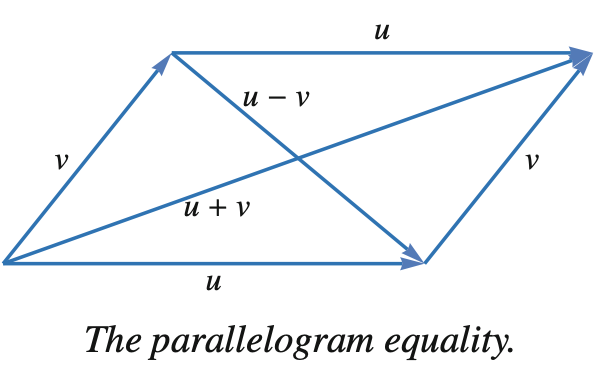
\includegraphics[width=0.25\textwidth]{axler6aparallelogram.png}
\end{figure}
\begin{proposition}[Parallelogram Equality]{}
  Suppose $u,v\in V$. Then \[
    \|u+v\|^2+\|u-v\|^2=2(\|u\|^2+\|v\|^2)
  .\] 
\end{proposition}
\begin{proof}[Proof]
  \begin{align*}
    \|u+v\|^2+\|u-v\|^2&= \left<u+v,u+v \right>+\left<u-v,u-v \right> \\
                       &= \|u\|^2+\|v\|^2+\left<u,v \right>+\left<v,u
                       \right>+\|u\|^2+\|v\|^2-\left<u,v \right>-\left<v,u \right>\\
                       &=2(\|u\|^2+\|v\|^2)
  ,\end{align*} as desired.
\end{proof}















\end{document}
